
% !TEX root = DesignDocument.tex

\chapter{Design  and Implementation}

The design of the cluster is going to change as we test different configurations to determine which is capable of producing the most gigaflops, and as we test different connection methods. This section will outline the different designs we have created, how they were implemented, and our plans for implementing future designs going forward.

%%
\begin{comment}
This section is used to describe the design details for each of the major components in the system.    Note that this chapter is critical for all tracks.  Research tracks would do experimental design here where other tracks would include the engineering design aspects.    This section is not brief and requires the necessary detail that can be used by the reader to truly understand the architecture and implementation details without having to dig into the code.    Sample algorithm:  Algorithm~\ref{alg1}.  This algorithm environment is automatically placed - meaning it floats.   You don't have to worry about placement or numbering.  

\begin{algorithm} [tbh]                     % enter the algorithm environment
\caption{Calculate $y = x^n$}          % give the algorithm a caption
\label{alg1}                           % and a label for \ref{} commands later in the document
\begin{algorithmic}                    % enter the algorithmic environment
    \REQUIRE $n \geq 0 \vee x \neq 0$
    \ENSURE $y = x^n$
    \STATE $y \Leftarrow 1$
    \IF{$n < 0$}
        \STATE $X \Leftarrow 1 / x$
        \STATE $N \Leftarrow -n$
    \ELSE
        \STATE $X \Leftarrow x$
        \STATE $N \Leftarrow n$
    \ENDIF
    \WHILE{$N \neq 0$}
        \IF{$N$ is even}
            \STATE $X \Leftarrow X \times X$
            \STATE $N \Leftarrow N / 2$
        \ELSE[$N$ is odd]
            \STATE $y \Leftarrow y \times X$
            \STATE $N \Leftarrow N - 1$
        \ENDIF
    \ENDWHILE
\end{algorithmic}
\end{algorithm}
Citations look like~\cite{Choset:2005:PRM, arkin2009governing, lavalle2006}  and~\cite{wiki:asimo,lumelsky:1987, nolfi2000evolutionary}.  These are done automatically.  Just fill in the database {\tt designrefs.bib} using the same field structure as the other entries.  Then pdflatex the document, bibtex the document and pdflatex twice again.  The first pdflatex creates requests for bibliography entries.
The bibtex extracts and formats the requested entries.  The next pdflatex puts them in order and assigns labels.  The final pdflatex replaces references in the text with the assigned labels.
The bibliography is automatically constructed.  
 \end{comment}

 \section{Architecture and System Design}
 %%This is where you will place the overall system design or the architecture.   This section should be image rich.  There is the old phrase {\it a picture is worth a thousand words}, in this class it could be worth a hundred points (well if you sum up over the entire team).   One needs to enter the design and why a particular design has been done.   
 %% Andrew labeled this secion as Cluster Configure in our old template
The first architecture we implemented was a star topology, with each device of the eight devices connected over Ethernet to a central switch. Each device was configured to be on the same network and capable of communicating over the switch via IP addresses. We configured the /home directory of our head node, Snow White, to be an NFS export that the seven other nodes would mount in their /home directory. This allowed for any change to be made on one device to be mirrored on the others. Also, it allowed for MPI programs located anywhere in the /home directory to be run, as all the devices would see the same executable in the same path.

\begin{figure}[h]
	\caption{Star topology.}
	\centering
		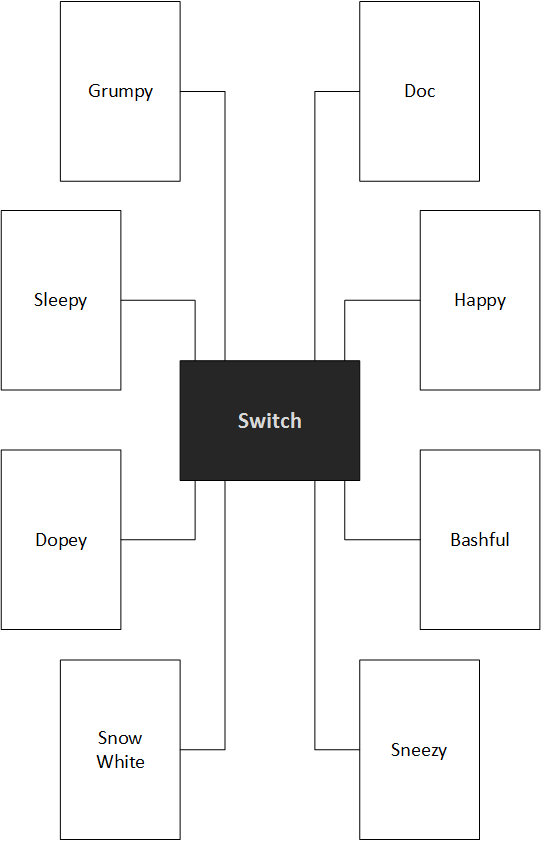
\includegraphics[scale=0.5]{cluster_star.png}
\end{figure}

	The next tolopogy we implemented was a ring. A USB to Ethernet device was attached to each ODroid, giving them a total of two network interfaces. Each interface was assigned a unique IP address, as shown in Figure Yada. This allowed the cluster to be connected without the switch, and instead with each ODroid connected to the ajacent two forming a ring. For communication to be possible, routing information had to be specified to allow each device to know the path to follow to connect to the other seven. To do this, the /etc/networking/interfaces file was edited to add seven routes, four from one network interface and three from the other. Each route specified which port to use to next to go to any given ODroid. For instance, Snow White had a route with the information that if any program tries to access Sleepy on 192.168.0.3, it would go through Dopey at 192.168.0.1, and then Dopey had it's own routing table for how to access Sleepy.
	The routing tables were designed such that each ODroid would take the fewest possible hops to get to any other. When the ODroids were equidistant, such as Snow White to Doc where going clockwise or counter-clockwise would each take four hops, the convention used was to go clockwise. This would allow the network traffic to overlap as little as possible in order to maximize effeciency. Therefore, each ODroid had a unique routing table. 

\begin{figure}[h]
	\caption{IP addresses for ring topology.}
	\centering
		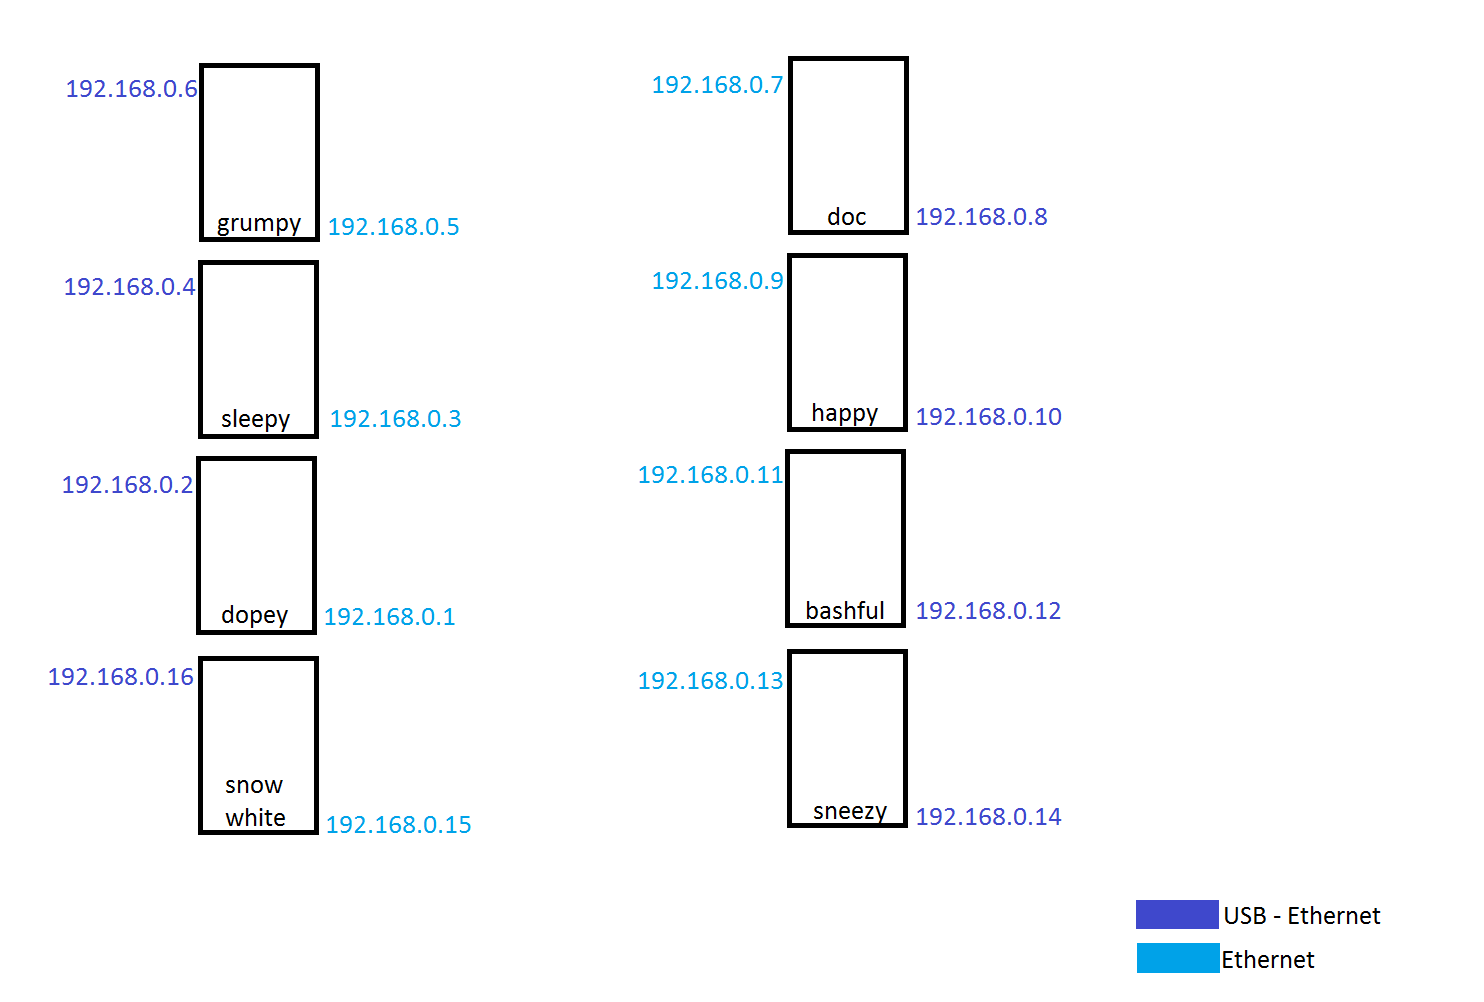
\includegraphics[scale=0.5]{cluster_ipaddresses.png}
\end{figure}

	The third architecture we used was a hypercube topology. To implement it, a third network interface was added by connecting a second USB to Ethernet device on the final USB 3.0 port. An IP address was assigned to that interface as well, and more routing table information was added. This allowed more connections to be made, decreasing the maximum amount of hops needed to get from any one node to another, as shown in Figure Blada. 

\begin{figure}[h]
	\caption{Diagram of hypercube topology.}
	\centering
		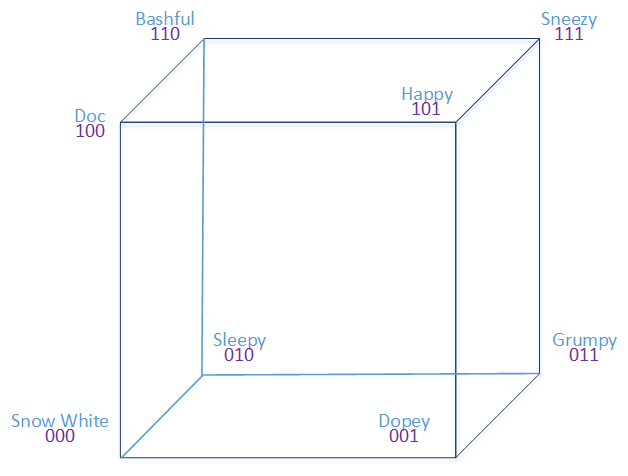
\includegraphics[scale=0.5]{HyperCube2.png}
\end{figure}


 \subsection{Design Selection}
 %%Failed designs, design ideas, rejected designs here.
	For the purposes of benchmarking the cluster, the star topology was used. It was found that MPI does not work with multiple network interfaces on the same subnet existing on the same node. It also did not work on our cluster even when the IP addresses were changed so that the networks were on different subnets. Therefore, in order to be able to use the benchmarking tool Linpack the star topology had to be used, as it was the only design that had only one network interface per ODroid.
 
 \subsection{Data Structures and Algorithms}
 %%Describe the special data structures and any special algorithms.
	

 \subsection{Data Flow}
	For this project, the most significant data flow was how LINPACK processes were distributed. The goal was to divide the work as much as possible, both across the cluster and within each device itself. In order to accomplish this, MPI was used with LINPACK to spawn as many processes as needed and run them on different cores. 
 
 \subsection{Communications}
	To communicate between devices, many different methods were tested. First, Ethernet communication through a switch was used to set up the initial cluster. The communication was configured by setting each port with a static IP address to allow the devices to exist on the same network. Communication could then occur through the switch very easily, as each device was physically connected to each other device. 
	USB and GPIO communication were also tested. USB to USB was found to be impossible due to USB 3.0 host to host communication being not supported by any existing operating system. GPIO communication was successful using WiringPi with C code. However, it was found to be much slower than Ethernet, and creating any type of large scale communication efforts would have been beyond the scope of this project.
 
 \subsection{Classes}
 
 \subsection{UML}

\section{Major Component \#1 }

\subsection{Technologies  Used}
%%This section provides a list of technologies used for this component.  The details for the technologies have already been provided in the Overview section.
	 

\subsection{Component  Overview}
%%This section can take the form of a list of features. 

\subsection{Phase Overview}
%%This is an extension of the Phase Overview above, but specific to this component. It is meant to be basically a brief list with space for marking the phase status. 

\subsection{ Architecture  Diagram}
%%It is important to build and maintain an architecture diagram.  However, it may be that a component is best described visually with a data flow diagram. 


\subsection{Data Flow Diagram}
%%It is important to build and maintain a data flow diagram.  However, it may be that a component is best described visually with an architecture diagram. 


\subsection{Design Details}
%%This is where the details are presented and may contain subsections.   Here is an example code listing:
First, we made the devices able to communicate on the same network. We assigned each device a static IP address by editing the /etc/networking/interfaces file to incluce the IP address chosen for the device. All addresses were on the 192.168.1.X network, and the last number was 11 through 18 for the eight devices.

Next, we set each device to be able to use our naming convention in place of an IP address for any purpose, such as by using "ssh sleepy" instead of "ssh 192.168.1.13". To do this, we changed the /etc/hostname file to replace "odroid" with the name we wanted, and added entries to /etc/hosts to include the IP address of the other seven decives. 

We then set the /home directory of Snow White to be an NFS share that could be mounted on the dwarfs. After nfs-kernel-server was installed on Snow White, we edited it's /etc/exports file to include /home as an export. The dwarfs then installed nfs-common and used the command "mount SnowWhite:/home /home" to mount the home directory of Snow White over their own.

To make this mount process automatic on boot, we edited the /etc/fstab file on each dwarf to make them mount Snow White's home directory as part of the boot process. This proved unsuccesful, however, on all devices except for on. As a work around, we wrote a Python tool that can be run from Snow White to mount it's home directory on the dwarfs.

\begin{lstlisting}
#!/bin/usr/python

import os

def Main():

        hosts = [ 'snow_white', 'dopey', 'sleepy', 'grumpy', 'doc', 'happy',
 				  'bashful', 'sneezy' ]

        for host in hosts:
                if host != 'snow_white':
                        cmd = "ssh odroid@" + host + " 'sudo mount -t nfs snow_white:/
							   home /home'"
                        os.system( cmd )

if __name__ == '__main__':
        Main()
\end{lstlisting}
%%This code listing is not floating or automatically numbered.  If you want auto-numbering, but it in the algorithm environment (not algorithmic however) shown above.

\section{Major Component \#2 }

\subsection{Technologies  Used}
%%This section provides a list of technologies used for this component.  The details for the technologies have already been provided in the Overview section. 

\subsection{Component  Overview}
%%This section can take the form of a list of features. 

\subsection{Phase Overview}
%%This is an extension of the Phase Overview above, but specific to this component. It is meant to be basically a brief list with space for marking the phase status. 

\subsection{ Architecture  Diagram}
%%It is important to build and maintain an architecture diagram.  However, it may be that a component is best described visually with a data flow diagram. 


\subsection{Data Flow Diagram}
%%It is important to build and maintain a data flow diagram.  However, it may be that a component is best described visually with an architecture diagram. 


\subsection{Design Details}
%%This is where the details are presented and may contain subsections. 


\section{Major Component \#3 }

\subsection{Technologies  Used}
%%This section provides a list of technologies used for this component.  The details for the technologies have already been provided in the Overview section. 
We used several Linux system configuration tools to implement the cluster. We used the files
\begin{itemize}
	\item etc/network/interfaces
	\item etc/exports
	\item etc/hostname
	\item etc/hosts
	\item etc/fstab
\end{itemize}
for several different configuration setting. We also used a few packages availible from the defual debian repositories.
\begin{itemize}
	\item nfs-kernel-server
	\item nfs-common
	\item mpi-dev
\end{itemize}

Finally, we used SSH tools that are installed by default on Ubuntu 15.


\subsection{Component  Overview}
%%This section can take the form of a list of features. 
The features implented by this configuration were:

\begin{itemize} 
	\item All devices recognizing the others over Ethernet.
	\item SSH without requiring a password.
	\item Mount home directory of Snow White on the dwarfs.
	\item Running MPI code on all devices.
\end{itemize}


\subsection{Phase Overview}
%%This is an extension of the Phase Overview above, but specific to this component. It is meant to be basically a brief list with space for marking the phase status. 

\subsection{ Architecture  Diagram}
%%It is important to build and maintain an architecture diagram.  However, it may be that a component is best described visually with a data flow diagram. 


\subsection{Data Flow Diagram}
%%It is important to build and maintain a data flow diagram.  However, it may be that a component is best described visually with an architecture diagram. 


\subsection{Design Details}
%%This is where the details are presented and may contain subsections. 

